%
% The first command in your LaTeX source must be the \documentclass command.
\documentclass[sigconf,screen]{acmart}

%
% defining the \BibTeX command - from Oren Patashnik's original BibTeX documentation.
\def\BibTeX{{\rm B\kern-.05em{\sc i\kern-.025em b}\kern-.08emT\kern-.1667em\lower.7ex\hbox{E}\kern-.125emX}}
    
% Rights management information. 
% This information is sent to you when you complete the rights form.
% These commands have SAMPLE values in them; it is your responsibility as an author to replace
% the commands and values with those provided to you when you complete the rights form.
%
% These commands are for a PROCEEDINGS abstract or paper.
% \copyrightyear{2019}
% \acmYear{2018}
% \setcopyright{acmlicensed}
% \acmConference[Emsoft '19]{Emsoft '19: Embedded Systems Week}{Oct 13--18, 2019}{New York, NY}
% \acmBooktitle{Woodstock '18: Safe SCUBA Diving, June Oct 13--18, 2019, New York, NY}
% \acmPrice{15.00}
% \acmDOI{10.1145/1122445.1122456}
% \acmISBN{978-1-4503-9999-9/18/06}

%
% These commands are for a JOURNAL article.
%\setcopyright{acmcopyright}
%\acmJournal{TOG}
%\acmYear{2018}\acmVolume{37}\acmNumber{4}\acmArticle{111}\acmMonth{8}
%\acmDOI{10.1145/1122445.1122456}

%
% Submission ID. 
% Use this when submitting an article to a sponsored event. You'll receive a unique submission ID from the organizers
% of the event, and this ID should be used as the parameter to this command.
%\acmSubmissionID{123-A56-BU3}

%
% The majority of ACM publications use numbered citations and references. If you are preparing content for an event
% sponsored by ACM SIGGRAPH, you must use the "author year" style of citations and references. Uncommenting
% the next command will enable that style.
%\citestyle{acmauthoryear}

%
% end of the preamble, start of the body of the document source.
\usepackage{dL}
\usepackage{lsyntax}
\usepackage{lsemantics}
\usepackage{tablefootnote}
\usepackage{logic}
\usepackage{prettyref}
\usepackage{tikz,lipsum,lmodern}
\usepackage[most]{tcolorbox}



\newcommand{\varheart}{hr}
\newcommand{\vDesc}{\textit{vDesc}}
\newcommand{\vAsc}{\textit{vAsc}}
\newcommand{\tank}{\textit{tank}}
\newcommand{\tApprox}{\textit{tApprox}}
\newcommand{\iitimes}{{*}}
\newcommand{\stoppedTimer}{\textit{stoppedTimer}}
\newcommand{\stopTime}{\textit{stopTimer}}
\newcommand{\stopDepth}{\textit{stopDepth}}
\newcommand{\stoppedTimerEnabled}{\textit{stoppedTimerEnabled}}

\newcommand{\den}[1]{\llbracket#1\rrbracket}




\begin{document}

%
% The "title" command has an optional parameter, allowing the author to define a "short title" to be used in page headers.
\title{Safe SCUBA Diving}

%
% The "author" command and its associated commands are used to define the authors and their affiliations.
% Of note is the shared affiliation of the first two authors, and the "authornote" and "authornotemark" commands
% used to denote shared contribution to the research.
\author{Viren Bajaj}
% \authornote{Both authors contributed equally to this research.}
\email{vbajaj@alumni.cmu.edu}
% \orcid{1234-5678-9012}
\affiliation{%
  \institution{Carnegie Mellon University}
  \streetaddress{5000 Forbes Avenue}
  \city{Pittsburgh}
  \state{Pennsylvania}
  \postcode{15213}
}

\author{Nathan Fulton}
\email{nrfulton@cs.cmu.edu}
\affiliation{%
  \institution{Carnegie Mellon University}
  \streetaddress{5000 Forbes Avenue}
  \city{Pittsburgh}
  \state{Pennsylvania}
  \postcode{15213}
}


\author{Andre Platzer}
\affiliation{%
  \institution{Carnegie Mellon University}
  \streetaddress{5000 Forbes Avenue}
  \city{Pittsburgh}
  \state{Pennsylvania}
  \postcode{15213}
}

\author{Kareem Elmaroufi}
\affiliation{%
  \institution{Carnegie Mellon University}
  \streetaddress{5000 Forbes Avenue}
  \city{Pittsburgh}
  \state{Pennsylvania}
  \postcode{15213}
}
 


%
% By default, the full list of authors will be used in the page headers. Often, this list is too long, and will overlap
% other information printed in the page headers. This command allows the author to define a more concise list
% of authors' names for this purpose.
\renewcommand{\shortauthors}{Trovato and Tobin, et al.}

%
% The abstract is a short summary of the work to be presented in the article.
\begin{abstract}
SCUBA diving is a safety critical activity because changing depth too rapidly or running out of oxygen before surfacing can result in life-threatening consequences. SCUBA divers are trained to circumvent these issues by monitoring their rate of ascent, descent, and air consumption using a wrist-mounted computer. 
These dive computers measure air consumption using a pressure gauge fixed on the tank that connects to it via a wireless transmitter. Unfortunately, this method is often considered prohibitively expensive and creates an additional point of failure in a safety-critical system.
To deal with these two issues, we present a hybrid systems model of a SCUBA diving computer that uses a commodity heart rate sensor to estimate air consumption. We formally verify this model to ensure that the diver surfaces without running out of air even when a safety stop is necessary.
\end{abstract}

%
% The code below is generated by the tool at http://dl.acm.org/ccs.cfm.
% Please copy and paste the code instead of the example below.
%
\begin{CCSXML}
<ccs2012>
 <concept>
  <concept_id>10010520.10010553.10010562</concept_id>
  <concept_desc>Computer systems organization~Embedded systems</concept_desc>
  <concept_significance>500</concept_significance>
 </concept>
 <concept>
  <concept_id>10010520.10010575.10010755</concept_id>
  <concept_desc>Computer systems organization~Redundancy</concept_desc>
  <concept_significance>300</concept_significance>
 </concept>
 <concept>
  <concept_id>10010520.10010553.10010554</concept_id>
  <concept_desc>Computer systems organization~Robotics</concept_desc>
  <concept_significance>100</concept_significance>
 </concept>
 <concept>
  <concept_id>10003033.10003083.10003095</concept_id>
  <concept_desc>Networks~Network reliability</concept_desc>
  <concept_significance>100</concept_significance>
 </concept>
</ccs2012>
\end{CCSXML}

\ccsdesc[500]{Computer systems organization~Embedded systems}
\ccsdesc[300]{Computer systems organization~Redundancy}
\ccsdesc{Computer systems organization~Robotics}
\ccsdesc[100]{Networks~Network reliability}

%
% Keywords. The author(s) should pick words that accurately describe the work being
% presented. Separate the keywords with commas.
\keywords{hybrid systems, formal verificaiton, IoT, human-in-the-loop controller}

%
% A "teaser" image appears between the author and affiliation information and the body 
% of the document, and typically spans the page. 
% \begin{teaserfigure}
%   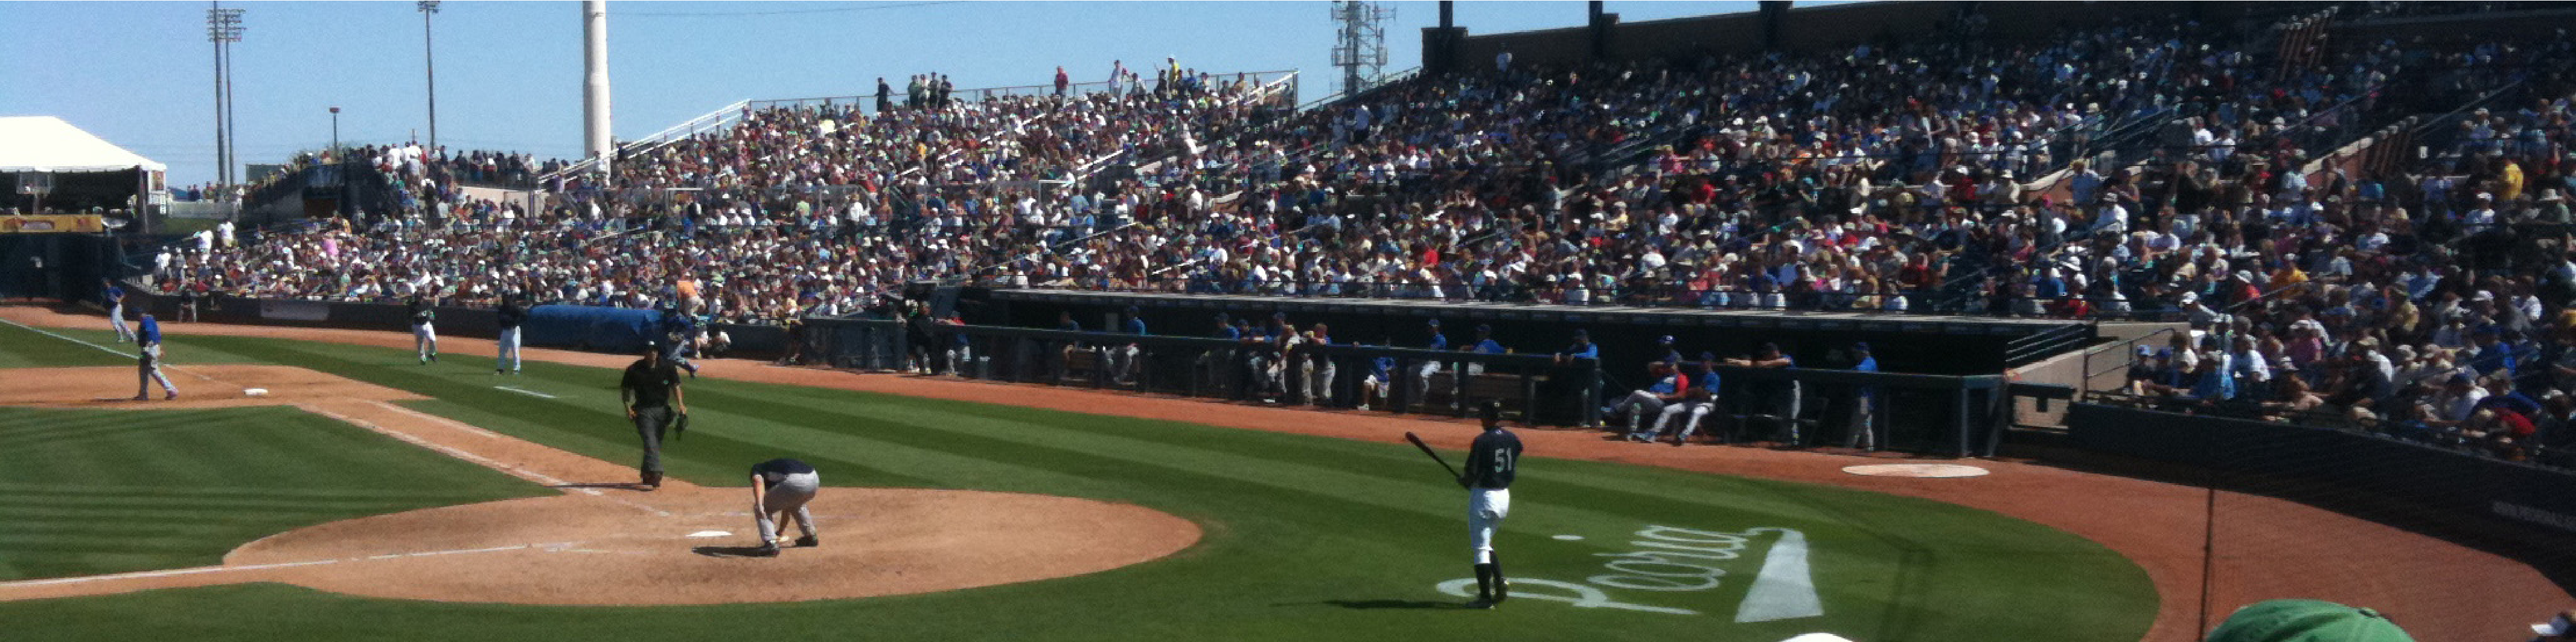
\includegraphics[width=\textwidth]{sampleteaser}
%   \caption{Seattle Mariners at Spring Training, 2010.}
%   \Description{Enjoying the baseball game from the third-base seats. Ichiro Suzuki preparing to bat.}
%   \label{fig:teaser}
% \end{teaserfigure}

%
% This command processes the author and affiliation and title information and builds
% the first part of the formatted document.
\maketitle

\section{Introduction - todo}




% \section{Background}
%  This section reviews the physiological underpinnings of our model - the mathematical relation between heart rate and air consumption.
 
%  Hybrid programs, a programming language for hybrid systems; differential dynamic logic (\dDL) for specifying reachability properties about hybrid programs; and the theorem prover KeYmaera X for \dDL have been explained in the appendix.
 
% \subsection{Heart Rate Kinetics and Oxygen Uptake}

% To be able to estimate air consumption using a heart rate sensor, it is critical to understand the dynamics of heart rate and how it relates to air consumption. 

% Stirling et. al. provide a convincing model of heart rate kinetics which relates heart rate to exercise intensity. As divers tend not to perform sustained vigorous movements, it is reasonable to assume that they stay below the lactate threshold. This assumption allows us to use the simplified equation:
% $hr' = b(hr_{ss} - hr)$ where hr is the heart rate, $hr_{ss}$ is the steady state heart rate that is asymptotically reached as a result of exercise intensity. 

 
% [?] note that the relationship between percentage of maximal heart rate and percentage of maximal oxygen consumption can be modeled by a linear function, but the coefficients on this function must be experimentally determined and vary between fitness groups and sexes. 

% Combining these two insights, we create a conservative model relating heart rate to oxygen consumption that is parametric in the exact choice of coefficients. We achieve this design flexibility by leaving several coefficients in our model unspecified so that these can be experimentally determined on a per-user basis. The ability to verify a system with symbolic constraints rather than specifying a priori bounds for system parameters is one motivation for choosing KeYmaera X instead of SpaceEx [?], FLOW* [?], or dReal/dReach [?].

% [?] introduce specialized and high-fidelity models of the human heart. We use a much less fine-grained model because most of our model’s conservativism comes from the relationship between heart rate dynamics and oxygen consumption/demand, rather than from coarse-grained modeling of the heart itself.

% [?] suggests that the relationship between heart rate and oxygen consumption could be determined using machine learning techniques. This paper considers a first-principles model, but notice ? demonstrate how KeYmaera X is able to use first-principles models to inform and provide safety guarantees for machine learning algorithms.

\section{The Model}

The primary contribution of this paper is a model (Fig 1) of a hybrid dynamical system consisting of a scuba diver and depth and heart rate sensors. The model captures the behavior of the diver, and dynamics of depth and heart rate, which is used to show that the diver does not: 1) run out of air before surfacing and 2) completes a safety stop to avoid decompression sickness. These safety critical properties are proven for all initial configurations of the model parameters, which are constrained to physiologically and mathematically realistic domains.

This section explains some of our important 
modelling choices.

\subsection{Dynamics}
A hybrid system must account for all possible evolutions of variables in between sensor measurements, in order to be verifiable. 

We capture the evolution of heart rate based on a convincing model of heart rate kinetics proposed by Stirling et. al. which relates heart rate to exercise intensity. By making the simplifying assumption that divers stay below the lactate threshold, since they tend not to make vigorous movements, we can use the equation:
$hr' = b(hr_{ss} - hr)$. Where hr is the heart rate, b is a positive constant, and $hr_{ss}$ is the steady state heart rate that is asymptotically reached in order to meets the demands imposed by exercise intensity.

To understand the evolution of the volume of air in the tank we rely on a study that subjected 81 men and women between the age of 18 and 34 to an incremental exercise test to exhaustion and found a linear relationship between percentage of maximum heart rate and percentage of maximum oxygen consumption. \footnote[2]{the coefficients on this function ($\tau$ in our model) must be experimentally determined and vary between fitness groups and sexes.} Since the maximum oxygen consumption is an upper bound on the rate of depletion of air from the tank, we can model its dynamics as $tank' = - \tau * \varheart$

Using this system of coupled ordinary differential equations, we create a conservative model relating heart rate to oxygen consumption that is parametric in the exact choice of coefficients. We achieve this design flexibility by leaving several coefficients i
n our model unspecified so that these can be experimentally determined on a per-user basis. The ability to verify a system with symbolic constraints rather than specifying a priori bounds for system parameters is one motivation for choosing KeYmaera X instead of SpaceEx [?], FLOW* [?], or dReal/dReach [?].

\subsection{Behavior}
The hybrid program behavior describes the set of actions that a diver may take, namely, ascend, descend or stay at their current depth. Rather than prescribing a concrete action that the diver must take at any given moment, this model specifies the \textbf{system configurations} (through assignments and tests - show this in the visual) in which the diver may choose one of the actions, thereby making the model highly nondeterministic. 

This specification can be implemented in many different ways, e.g., a dive computer could beep whenever detecting a state where the diver must begin their ascent. Since divers are advised to limit their rate of vertical movement to 10 m/s, we assume the ascent and descent velocity to be a constant value. 

Each component of the behavior program contains tests which indicate conditions that must be true if the diver chooses to take the associated action. For example, in \textit{descend} the dive computer will check three conditions, two of which are discussed below and one is discussed in sec [safety stop]

\begin{enumerate}
    \item 
        \begin{align*}
            \tApprox &>\tau \varheart_{\text{max}} C + \tau \varheart_{\text{max}}\frac{-d - C \iitimes \vDesc}{\vAsc} \\ &+ \tau \varheart_{\text{max}}(stopDuration - stoppedTime);
        \end{align*}
which states that the tank contains enough oxygen to allow the diver
1) to descend for $c \le C$ seconds
2) ascend to the surface from their new depth ($d = d_0 + c\iitimes\vDesc$) and,
3) to stop for the remaining time of the stopDuration.

    \item 
        $$?\varheart_{min} \le \varheart_{ss} \le \varheart_{max};$$
which states that the diver's steady state heart rate (or equivalently, level of exertion) is physically realizable. 
% i.e., the diver will not approach an impossibly low or impossibly high heart rate.
Notice that our model allows the diver to directly choose their vertical velocity,
\footnote[1]{We elide  acceleration and jerk from our model for two reasons.
First, divers can accelerate and decelerate quickly enough that modeling these variables isn't necessary. Second, the addition of acceleration adds nothing of scientific interest to our modeling formalism; the treatment of second and third derivatives is already well-studied.}
but never a particular level of exertion ($\varheart_{ss} := *$).
%; e.g., by \cite{DBLP:conf/rssrail/MitschGBGP17,DBLP:journals/sttt/QueselMLAP15,DBLP:conf/icfem/PlatzerQ09}.
This is an important modeling choice because some factors
that effect exertion are not directly controllable, i.e., most humans cannot \emph{choose} their heart rate.
\end{enumerate}
If the first constraint is false, the dive computer can, e.g., display a ``Do Not Descend" advisory to the user.
We assume the diver obeys all such advisories. If no advisory is issued, the diver may choose to descend ($v := \vDesc$).

Another crucial aspect of our model is that none of these tests directly mention the tank volume (\textit{tank}). Directly testing the value of tank would correspond to directly sensing the volume of oxygen in the diver's tank; however, the entire point of our model is that we do not rely on having such a sensor. Instead, we use an approximation of the tank volume (\textit{tApprox}). This approximation is computed by making worst-case assumptions about the diver's future rate of oxygen consumption; these worst-case assumptions are necessary because (most) humans cannot directly control their heart rate (or, by extension, oxygen consumption). The hybrid program updateApprox updates the controller's approximation tApprox of the tank's volume \textit{t}.

% \subsubsection{Motion}

% \subsubsection{Safety Stop}
\subsection{Ground truth update}
The basic model relies on a very poor approximation of oxygen consumed between each control step.
Some over-approximation is necessary because we can't know, for certain, how the diver's heart rate
changes in-between sensor measurements. To compensate, we modify the basic model in a way that allows
the diver to occasionally manually update the tank approximation with ground truth about the amount of oxygen in the tank.

The \textit{groundTruthUpdate} program models a choice $\cup$, made by the diver at each control step, between continuing with the current tank approximation ($\tApprox := \tApprox$) or updating the tank's approximation with the ground truth
($\tApprox := t$). The former program is equivalent to the empty program, i.e., a no-op.

A concrete implementation of this update is, e.g., the diver looking at an analog read-out of the oxygen remaining in their tank
and inputting this value into their dive computer.


\subsection{Safety Stop}
To be complete our model must account for a decompression stop that divers often need to make to avoid decompression sickness. Our model allows the diver to stop for a pre-specified duration (\textit{stopDuration}) at a pre-specified depth (\textit{stopDepth}  based on the dive plan \footnote[2]){The stop depth is always prescribed to be between 15-20 feet.}.

The system of differential equations is extended with two event triggers, one which triggers the controller when the diver arrives at the stop depth,
and one that triggers the controller when the $\stopTime$ has elapsed. Both of these event-triggers could be implemented using auditory or
visual cues (e.g., a beeping sound together with an appropriate message on the diver's wrist computer).

The first test in the stay case and the descend case are modified to ensure that the diver has enough oxygen to
reach the surface \textbf{even after performing a safety stop} at the specified depth ($\stopDepth$) and for the
specified amount of time ($\stopTime$).

The $\stoppedTimerEnabled$ variable tracks whether the diver is currently stopped.
The timer is only enabled (i.e., equal to $1$) when the diver is currently stopped at the specified $\stopDepth$.
Notice that the diver may stay still / move horizontally even if the timer is not enabled.
This behavior is implemented by the additional test at the bottom of the stay case;
an choice turns on the $\stoppedTimer$ if the diver is currently at the
$\stopDepth$, and otherwise does not turn on the $\stoppedTimer$.

The diver is only allowed to ascend once the safety stop is complete ($\stoppedTimer = \stopTime$), \emph{or} if the diver has not already
reached the stop depth ($d > \stopDepth$).



\subsection{Initial configuration and Conclusion}
The \textit{init} formula describes the system's initial configuration,
including bounds on system parameters and a description of safe starting configurations for other variables.

\begin{table*}
  \caption{Model Variables and Constraints}
  \label{tab:vars}
  \begin{tabular}{lll}
    \toprule
    Variable & Meaning & Constraints\\
    \midrule
    hr & Heart rate & $hr_{min}<hr<hr_{max}$\\
    $hr_{min}, hr_{max}$ & Physiological limits on hr & $0<hr_{min}<hr_{max}$\\
    $hr_{ss}$ & Steady state hr & $hr_{min}<hr<hr_{max}$\\
    $\tau,b$ & Parameters fit to diver& $>0$\\ \hline
    d & Depth & $>0$\\
    v & Current velocity & - \\
    vDec& Descent velocity & +15m/s\\ 
    vAsc & Ascent velocity & -15m/s\\ \hline 
    tank & Volume of air in tank & - \\
    tApprox & Controller's approximation of tank & - \\ \hline
    c & Time since previous control step & $\geq0$\\
    C & Maximum time between control steps & $>0$\\ 
  \bottomrule
\end{tabular}
\end{table*}

\section{Safety Theorem}


\section{Citations and Bibliographies}

%
% The acknowledgments section is defined using the "acks" environment (and NOT an unnumbered section). This ensures
% the proper identification of the section in the article metadata, and the consistent spelling of the heading.
% \begin{acks}
% To Robert, for the bagels and explaining CMYK and color spaces.
% \end{acks}

%
% The next two lines define the bibliography style to be used, and the bibliography file.
\bibliographystyle{ACM-Reference-Format}
\bibliography{sample-base}

% 
% If your work has an appendix, this is the place to put it.
\appendix

\section{Hybrid Systems}
Hybrid (dynamical) systems are mathematical models for analyzing the interaction between discrete and continuous dynamics. They are usually used to model technological systems whose logic and computation is dependent on the physical processes. A simple example of a hybrid system would be a thermostat which whose discrete state, on or off, depends on the continuously varying physical quantity, temperature.

\section{Hybrid programs}

Hybrid programs, introduced by ???, are a programming language for hybrid systems. Their syntax and informal semantics is given in Table X.
\begin{table}
  \caption{Hybrid Programs: Syntax and Semantics} \label{tab:hps}
  \begin{tabular}{l l}
    \toprule
    Program Statement & Meaning \\
    \midrule
    $\alpha;\beta$ & Sequentially composes $\beta$ after $\alpha$. \\
    $\alpha \cup \beta$ & Executes either $\alpha$ or $\beta$ \\ & nondeterministically.\\
    $\alpha^*$ & Repeats $\alpha$ zero or more times \\& nondeterministically.\\
    $x := \theta$ & Evaluates term $\theta$ and assigns result to $x$. \\
    $x := *$ & Assigns an arbitrary real value to $x$. \\
    $\{x_1'=\theta_1,...,x_n'=\theta_n \& F\}$ & Continuous evolution\footnotemark. \\
    $?F$ & Aborts if formula $F$ is not true.\\
    \bottomrule
  \end{tabular}
\end{table}
  \footnotetext{A continuous evolution along the differential equation system $x_i'=\theta_i$ for an arbitrary duration within the region described by formula $F$.}
  
To illustrate, Example 1 is a hybrid program representing a SCUBA divers vertical movement. The discrete choice of ascending, staying, or descending, drives their depth which is changing continuously with time. This differential equation is assumed to evolve for an arbitrary amount of time $>=0$, such that the evolution domain constraint $d>=0$, is true throughout its evolution. This composition of the diver's discrete choice, followed by time evolution of their depth, may repeat arbitrarily many times as indicated by the repetition operator *.
\begin{example}[Simple model of a diver ascending or descending]
\label{ex:simpleDiver}
\[
    \prepeat{
      \big(\underbrace{(v{:=}vAsc \cup v{:=} 0 \cup v{:=}vDesc)}_{\textit{ctrl}}\ ;
      \underbrace{\{d'{=}v \& d \ge 0\}}_{\textit{plant}}\big)
    }
\]

% \rref{ex:simpleDiver} is a very simple model of the diver's vertical movement, eliding any details about oxygen consumption,
% safety stops, etc. This model allows the diver to either ascend ($av < 0$) or else descend ($dv > 0$) from
% his current depth ($d$). 
% This process may repeat arbitrarily many times (indicated by the repetition operator $\prepeat{}$). 
% Because there is an evolution domain constraint on $plant$, each continuous evolution many only continue for an arbitrary non-negative duration $r \in \reals$
% such that $d \ge 0$ is true throughout the flow of the differential equation.
% Any use of the $'$ operator in a hybrid program denotes the time derivative of the primed variable, term, or formula.
\end{example}

A hybrid program that models the heart rate can be seen in example 2. Since a human doesn't have explicit control over their heart rate, it is modeled as a non-deterministic assignment operator, followed by a 'test' which ensures the value assigned is within the physically realizable limits. This discrete state then determines the evolution of the heart rate, which is discussed in section [].

\begin{example}[Simple model of Heart Rate]
\label{ex:simpleHR}
\[
    \prepeat{
      \big(\underbrace{hr_{ss}{:=}*;?hr_{min}\leq hr_{ss}\leq hr_{max}}_{\textit{ctrl}}\ ;
      \underbrace{\{hr'{=}b(hr_{ss}-hr)\}}_{\textit{plant}}\big)
    }
\]
\end{example}


\section{Differential Dynamic Logic}
Differential dynamic logic ($\dDL$) is a first-order multimodal logic for specifying and prov- ing properties of hybrid programs. Each hybrid program $\alpha$ is associated with modal operators $[\alpha]$ and $\langle \alpha \rangle$, which express state reachability properties of the parametrizing program. The formula $[\alpha]\phi$ states that the formula $\phi$ is true in any state reachable by the hybrid program $\alpha$. Similarly, $\langle \alpha \rangle \phi$ expresses that the formula $\phi$ is true after some execution of $alpha$. The \dDL formulas are generated by the grammar:
$$ \phi :: = \theta_1 \sim \theta_2 | \neg \phi | \phi \wedge \psi | \phi \rightarrow \psi | \forall x \phi | \exists x \phi | [\alpha]\phi | \langle \alpha \rangle \phi  $$
where $\theta_i$ are arithmetic expressions over the reals, $\phi$ and $\psi$ are formulas, $\alpha$ ranges over hybrid programs, and $\sim$ is a comparison operator $=,\neq, \geq, >,\leq, <$. The quantifiers quantify over the reals. We denote by $s \models P$ the fact that P is true in state s; e.g., we denote by $s \models [\alpha]P$ the fact that $(s, t) \in \imodel[]{}{\alpha}$ implies $t \models P$ for all states t. When P is true in every state (i.e., valid) we simply write |= P.
Reachability properties for hybrid programs are expressible as \dDL formulas. ... 


\section{KeYmaera X}

is an axiomatic theorem prover for dL first introduced by ?. KeYmaera X provides a small axiomatic core, ensuring that results obtained from the prover can be trusted. In addition to a small core, KeYmaera X provides a proof programming language called Bellerophon for establishing verification results about hybrid programs ?.



\section{ Model }
\begin{align*}
\underbrace{t \ge 0 \land \dotsm \vphantom{\dibox{}}}_{\text{precondition}} & 
\limply 
\dibox{\prepeat{ \{ ctrl;
\{ \underbrace{\textit{ascend} \cup \textit{stay} \cup \textit{descend}}_{\text{diver's behavioral model}} \}; plant 
\}
}}\underbrace{\textit{tank} \ge 0}_{\text{postcondition}}
\label{eq:carmodel}
\end{align*}

\begin{tcolorbox}[enhanced,
  colback=blue!5!white,colframe=blue!75!black,colbacktitle=red!80!black,
  title=program,fonttitle=\bfseries,
  boxed title style={size=small,colframe=red!50!black}, boxsep=.5mm ]
 
    \begin{tcolorbox}[enhanced,attach boxed title to top center={yshift=-3mm,yshifttext=-1mm},
      colback=blue!5!white,colframe=blue!75!black,colbacktitle=red!80!black,
      title=ctrl,fonttitle=\bfseries,
      boxed title style={size=small,colframe=red!50!black}, boxsep=.1mm ]
      $\{\texttt{NOP} \cup \humod{t_{worst}}{t}\}$
    \end{tcolorbox}

    \begin{tcolorbox}[enhanced,attach boxed title to top center={yshift=-3mm,yshifttext=-1mm},
      colback=blue!5!white,colframe=blue!75!black,colbacktitle=red!80!black,
      title=Behavior,fonttitle=\bfseries,
      boxed title style={size=small,colframe=red!50!black}, boxsep=.1mm ]
  
  
          \begin{tcolorbox}[enhanced,
          colback=blue!5!white,colframe=blue!75!black,colbacktitle=red!80!black,
          title=descend,fonttitle=\bfseries,boxed title style={size=small,colframe=red!50!black}, boxsep= .5mm ]
          $
          \{?t_{worst} \ge \tau*hr_{max} * \epsilon
                + \tau hr_{max}  \frac{-d - v_{desc}\epsilon}{v_{asc}};\\
                &\hspace{1.5cm}\humod{a}{*}; \humod{v}{0}\} 
            $
        \end{tcolorbox}
        \begin{tcolorbox}[enhanced,
          colback=blue!5!white,colframe=blue!75!black,colbacktitle=red!80!black,
          title=stay,fonttitle=\bfseries,boxed title style={size=small,colframe=red!50!black}, boxsep= .5mm ]
          $
          \{?t_{worst} \ge \tau hr_{max} \epsilon
                + \tau hr_{max}  \frac{-d}{v_{asc}};\\
                &\hspace{1.5cm}\humod{a}{*};\humod{v}{0}\}
            $
        \end{tcolorbox}
        \begin{tcolorbox}[enhanced,
          colback=blue!5!white,colframe=blue!75!black,colbacktitle=red!80!black,
          title=ascend,fonttitle=\bfseries,boxed title style={size=small,colframe=red!50!black}, boxsep= .5mm ]
          $$
          \{\humod{a}{*};\humod{v}{v_{asc}} \} 
            $$
        \end{tcolorbox}
    \end{tcolorbox}
    \begin{tcolorbox}[enhanced,attach boxed title to top center={yshift=-3mm,yshifttext=-1mm},
      colback=blue!5!white,colframe=blue!75!black,colbacktitle=red!80!black,
      title=plant,fonttitle=\bfseries,
      boxed title style={size=small,colframe=red!50!black}, boxsep=.1mm ]
     \begin{align*}
     \humod{c}{0};
          &\hspace{1.1cm}\{x' = b(a-x),\\
          &\ \hspace{1.1cm}t' = -\tau x,\\
          &\ \hspace{1.1cm}d' = v,\\
          &\ \hspace{1.1cm}c' = 1 \\
          &\ \hspace{1.1cm}\text{\& } d \ge 0 ~\land~c \le \epsilon\} \\
          &\hspace{1.1cm}\{\humod{t_{worst}}{t_{worst} - \tau hr_{max} c}\}
     \end{align*}
     
    \end{tcolorbox}
    
\end{tcolorbox}


\begin{align*}
\bm{ctrl} &\equiv \{\texttt{NOP} \cup \humod{t_{worst}}{t}\} \\\\
\bm{ascend} &\equiv \{\humod{a}{*};\humod{v}{v_{asc}} \} \\\\
\bm{stay} &\equiv \{?t_{worst} \ge \tau hr_{max} \epsilon
        + \tau hr_{max}  \frac{-d}{v_{asc}};\\
        &\hspace{1.5cm}\humod{a}{*};\humod{v}{0}\} \\\\
\bm{descend} &\equiv \{?t_{worst} \ge \tau*hr_{max} * \epsilon
        + \tau hr_{max}  \frac{-d - v_{desc}\epsilon}{v_{asc}};\\
        &\hspace{1.5cm}\humod{a}{*}; \humod{v}{0}\} \\\\
\bm{plant} &\equiv  \humod{c}{0}; \\
          &\hspace{1.1cm}\{x' = b(a-x),\\
          &\ \hspace{1.1cm}t' = -\tau x,\\
          &\ \hspace{1.1cm}d' = v,\\
          &\ \hspace{1.1cm}c' = 1 \\
          &\ \hspace{1.1cm}\text{\& } d \ge 0 ~\land~c \le \epsilon\} \\
          &\hspace{1.1cm}\{\humod{t_{worst}}{t_{worst} - \tau hr_{max} c}\} 
\end{align*} 
 
\end{document}
